\documentclass[10pt,a4paper]{IEEEtran}
\usepackage[latin1]{inputenc}
\usepackage[spanish]{babel}
\usepackage{amssymb}
\usepackage{graphicx}
\usepackage{float}
\usepackage{hyperref}
\usepackage{subcaption} 
\usepackage{amsmath}
\usepackage{amsfonts}
\usepackage[usenames]{color}
\author{Gatica, Isaias \\ Martin, Santiago \\ Saez, Lautaro �ndres \\ Vidman, Xavier Harry}
\title{Proyecto integrador DSP \\ Filtrado de ruido con transformada de wavelet}
\providecommand{\abs}[1]{\lvert#1\rvert}
\date{}

\begin{document}
\maketitle

\section{Introducci�n}
En el siguiente informe estudiaremos los conceptos de las se�ales wavelets, transformada de wavelet, y como utilizarlos para filtrar ruido de se�ales unidimensionales y bidimensionales.

\section{Marco te�rico}
Una \textit{Wavelet} es una ``peque�a onda'' que tiene su energ�a concentrada en un per�odo de tiempo determinado, son de duraci�n definida, irregulares,lo que les permite 
adaptarse y converger de mejor manera a la se�al que se quiere analizar.
Las familias de estas wavelet se definen como:
\begin{equation}
    \label{WM}
    \psi_{a,b}(t)= \frac{1}{\sqrt{a}} \psi(\frac{t-b}{a}) \quad a,b \in \mathbb{R} \quad ; a \not = 0. 
\end{equation}
Donde $a$ y $b$ son los par�metros de escala y traslaci�n respectivamente, se puede ver en la figura \ref{fig.a_b} como trabajan los par�metros $a$ y $b$. El par�metro $b$, asociado a la traslaci�n, hace que la wavelet recorra a la se�al $x(t)$ a trav�s del tiempo. Mientras que el par�metro $a$, permite controlar el ancho de la wavelet.

Por otro lado, la transformada de wavelet queda definida como:

\begin{equation}
C_{f} (a,b) = \int_{-\infty}^{+\infty} x(t) \overline{\psi_{a,b} (t)} dt
\end{equation}

Donde $\psi_{a,b}(t)$ es la funci�n que se utiliza para analizar a la se�al $x(t)$ que se quiera estudiar. Realizando una analog�a con Fourier, el trabajo que realiza $\psi_{a,b}(t)$, es an�logo al de las exponenciales complejas $e^{- j \omega t}$. El resultado de esta transformada es una familia de coeficientes  $C_{f} (a,b)$ que representan de mejor manera la se�al teniendo en cuenta la wavelet utilizada. Es notorio que el resultado es bidimensional ya que $a$ y $b$ son par�metros independientes. Donde $a$ esta relacionado con la frecuencia que posee la se�al y $b$ nos brinda informaci�n del momento temporal que se analiza. Esto no permite realizar un analisis en tiempo-frecuencia como se mencion� anteriormente. 
Cabe recalcar que existen diferentes tipos de wavelets madres, en la figura \ref{fig.wavelets_madres} se pueden ver las m�s utilizadas: 

\begin{figure}[htb]
	\centering
	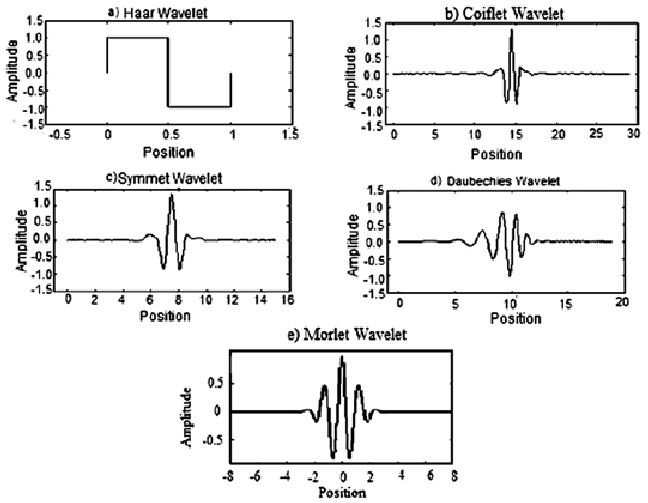
\includegraphics[width=.5\textwidth]{Fig/Wavelets}
	\caption{Bases ortonormales de wavelets madres m�s utilizadas}
	\label{fig.wavelets_madres}
\end{figure}

\begin{figure}[htb]
	\centering
	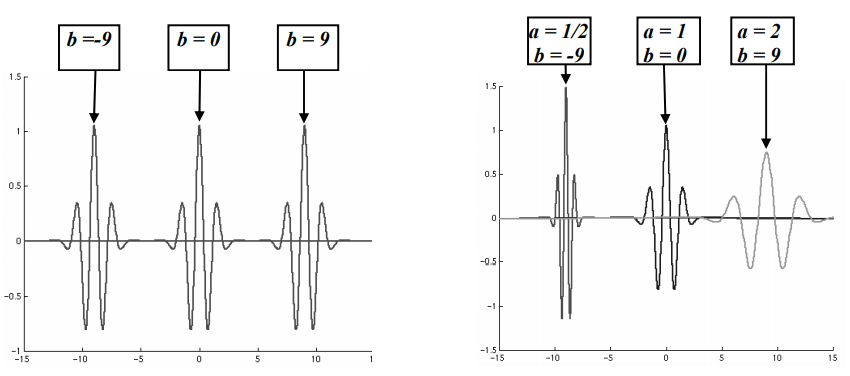
\includegraphics[width=.5\textwidth]{Fig/a_b}
	\caption{Traslaci�n y escalamiento de una wavelet}
	\label{fig.a_b}
\end{figure}

Debido a que los par�metros $a$ y $b$ pueden tomar infinitos valores se los limita utilizando el teorema de sampleo de Shanon para el cual:
\begin{align*} 
a=2\\ 
b=1
\end{align*}
Obteniendo la siguiente expresi�n para la familia de wavelet:
\begin{equation}
\psi_{j,k}(t) = 2^{-j/2} \psi (2^{-j}t-k)
\end{equation}
Para que esta funci�n $\psi$ sea una wavelet, las funciones $\{\psi_{j,k}\}_{\{j,k\} \in \mathbb Z }$ deben formar una base ortonormal de $L^2(\mathbb R)$. Con el fin de explicar este requerimiento es necesario explicar un concepto llamado Analisis Multi-Resoluc�on.

\subsection*{An�lisis Multi-Resoluci�n}
Un an�lisis multiresoluci�n para $L^{2}(\mathbb{R})$ consiste en una secuencia de subespacios cerrados de $L^{2}(\mathbb{R})$, $\{ V_{j} \}_{j \in \mathbb{Z} }$, y una funci�n $\phi \in V_{0}$ tal que se cumplan las siguientes condiciones: 

\begin{itemize}
\item[i] Los espacios $V_{j}$ est�n anidados, es decir:

\begin{equation*}
... \subset V_{-1} \subset V_{0} \subset V_{1} ...
\end{equation*}
\item[ii] $\overline{\cup _{j\in \mathbb Z}V_j} = L^2(\mathbb R)$ y $\cap {j\in \mathbb Z}V_j = {0}$


\end{itemize} 

Definimos a los espacios $V{j}$ como los espacios de aproximaci�n. Por otro lado, definimos a $W_j$ como el complemento ortogonal de $V_j$ en $V_{j-1}$ esto nos permite plantear la siguiente relaci�n:
\begin{equation}
\label{Central}
V_{j-1} = V_j \oplus W_j
\end{equation}

$W_j$ es llamado conjunto de detalle debido a que la proyecci�n ortogonal de la se�al en este espacio son los detalles y $V_j$ espacio de aproximaci�n ya que la proyecci�n ortogonal de la se�al sobre este espacio son las aproximaciones. Esto nos permite reescribir la ecuaci�n \ref{Central} como:
\begin{equation}
A_{j-1}(t) = A_j(t) + D_j(t) 
\end{equation} 
Donde $A_j(t)$ se define como:
\begin{equation}
A_j(t)=\sum_{k \in \mathbb Z} \beta _{j,k} \phi _{j,k}(t)
\end{equation}
Donde:
\begin{equation}
\beta _{j,k}= <x(t), \phi _{j,k}(t)>= \int_\mathbb R x(t) \phi_{j,k}(t)dt
\end{equation}


\end{document}